\documentclass[conference]{IEEEtran}
\IEEEoverridecommandlockouts
% The preceding line is only needed to identify funding in the first footnote. If that is unneeded, please comment it out.
\usepackage{cite}
\usepackage{amsmath,amssymb,amsfonts}
\usepackage{algorithmic}
\usepackage{graphicx}
\usepackage{textcomp}
\usepackage{xcolor}
\def\BibTeX{{\rm B\kern-.05em{\sc i\kern-.025em b}\kern-.08em
    T\kern-.1667em\lower.7ex\hbox{E}\kern-.125emX}}
\begin{document}

\title{Logistic Regression\\
%{\footnotesize \textsuperscript{*}Note: Sub-titles are not captured in Xplore and
%should not be used}
%\thanks{Identify applicable funding agency here. If none, delete this.}
}

\author{\IEEEauthorblockN{Pena Benafa}
\IEEEauthorblockA{\textit{Electronic Engineering} \\
\textit{University of Applied Science Hamm-Lippstadt}\\
Lippstadt, Germany \\
pena.benafa@stud.hshl.de}
}

\maketitle

\begin{abstract}

\end{abstract}

\begin{IEEEkeywords}
component, formatting, style, styling, insert
\end{IEEEkeywords}

\section{Introduction}
The pioneer of machine learning (ML) defined ML as a "field of study that gives computer the ability to learn without being explicitly programmed. \cite{bb1} ML is a subset of Artificial Intelligence with roots in computational statistics which focus on using computers to make predictions. Like humans that learn from experiences, the objective in ML is to create mathematical models that can be trained to make useful outputs (predictions) when fed with input or training data experiences). From these experiences, the ML models are tuned by optimization
algorithm to produce accurate predictions. The ML models are able to generalize what they have learned from the training data (previous experience) so that they can make accurate predictions for a new and unseen data.\cite{bb2}

\subsection{Types of Machine Learning Algorithms}
There are different types of ML algorithms that exist and are used to solve variety of problems.Based on the types of the problems being solved, ML algorithms can be grouped in three: supervised learning, unsupervised learning and reinforcement learning

\subsubsection{Supervised Learning}
Consider the equation of straight line (Eq 1), in ML studies commonly referred to as regression equation.
               
\begin{equation} 
\label{equ1}
y = mx+b 
\end{equation} 

Where :\\
y = dependent variable \\
m = slope of the regression equation\\
x = independent variable\\
b = constant of the equation

In supervised learning, the ML model is given training data containing y and x. The model learns the relationship between these, i.e., m and b. Afterwards, the model is given a test data that contains only y, from its experience discovering m and b, it can predict the y’s for each x. The classification of skin lesions according to malignancy is an example of this.\cite{bb3} Based on the value of the predicted label or dependent variable, supervised learning algorithms are further grouped into two, regression and classification. And logistic regression algorithm is an example of classification supervised ML algorithm.\\

\subsubsection{Unsupervised Learning}
Unlike supervised learning in which the training dataset of the ML model contains both the independent variables and dependent variable(s), in unsupervised learning, the training dataset contains only independent variables — x’s. The ML model learns the relationship between all the independent variables, and then groups them accordingly. An example of this is identifying and grouping customers which are high profit, high value or low-risk buyers.\cite{bb4} Unsupervised ML algorithms are grouped into the following: association, clustering and dimension reduction.

\subsubsection{Reinforcement learning}
Reinforcement learning is different from supervised and unsupervised learning, in which problem dataset will contain at least independent variable(s), instead in reinforcement learning, an agent and an environment are constructed. Through trial and error, the agent learns from its environment while optimizing some set objective function. After every performed action, depending on the set goal, the agent gets a reward, or punishment or nothing. The agent uses these to determine the optimal path
to the goal. The AlphaGo and AlphaZero are good examples of this \cite{bb3} and \cite{bb5}.

\subsection{Description of the Classification Problem}
One of the problems in supervised learning is classification problem. In this type of problem, ML model built using ML classification algorithms learns from a training datasets containing features or independent variables ie x’s, and dependent variables or labels or classes (as they referred to in this case) i.e y’s. After training, the test dataset containing only the features are ‘classified’ or grouped
according to what model has learned from the training dataset. The classes can be binary, true or false, spam or not spam, 0 or 1, dog or cat, male or female etc. Or the dependent variables can be multi-class, that is instead being 0 or 1, spam or not, there can be third, fourth….nth class. Example, classification of apps in the App Store, an app can be classified as one of these, social media, game, news, weather, media (audio, photo, video), educational, health and fitness, entertainment etc. In
this work, the focus shall be on binary class problems.

Here are some examples of ML algorithms used for solving classification problems:
\begin{enumerate}
\item Logistic Regression
\item Support Vector Machine
\item k-Nearest Neighbours
\item Decision Trees
\item Naive Bayes
\item Random Forest etc.
\end{enumerate}

\section{Logistic Regression}
Logistic regression estimates probabilities using logistic function to measure the relationship between independent variables and a categorical (binary or multi-class) dependent variables. During the training phase the ML model learns the relationship between categorical dependent variables and the independent variable(s). In the test phase, for a given x, the model makes prediction based on probability that the corresponding y value for that x, is "false" or “true”. The sum of the
probability for these two outcomes is 1, however, the y value would be "false" if the probability value for “false” is greater than “true”. As mentioned earlier, probability for the outcome is govern by logistic function.

\subsection{Logistic Function}
Visually the shape of the logistic curve is shaped like an “S" and it is also called sigmoid curve.
A sigmoid curve which shows a sufficient degree of smoothness is a bounded differentiable real function that is defined for all real input values that has a positive derivative. \cite{bb7} The curve starts low, has a period of acceleration, and then approaches a straight line that defines the limit of a curve (asymptote).

\begin{figure}[h]
    \centering
    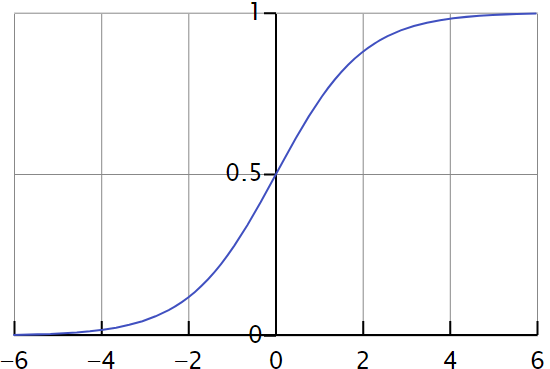
\includegraphics[scale=0.62]{figs/Lfunction.png}
    \caption{Graph of the standard logistic sigmoid function \cite{img}}
    \label{dabc}        
\end{figure}

\begin{equation} 
\label{equ2}
f(x) = \frac{L}{1 + e{^{-k(x-x0)}}}
\end{equation} 


Where:\\
L = the curves maximum value or the carrying capacity\\
k = the curves steepness or logistic growth rate\\
x = the independent variable\\
x0 = value of x at sigmoid’s midpoint\\

The maximum value of f(x) is obtained when it approaches L, that is when x approaches $+\infty$. And the minimum value of f(x) is obtained when it approaches zero, that is when x approaches $-\infty$.

\subsection{Examples}

\subsection{Dependent Variables}

\subsection{Independent Variables}


\section{Logistic Regression Model}

\subsection{Regression Equation}

\subsection{Regression Curve}
\subsection{Decision Boundary}
\subsection{Non-Linear Decision Boundary}

\section{Cost Function and Gradient Descent}

\section{Over fitting Problem}
\subsection{Under Fitting}
\subsection{Over Fitting}

\section{Regularized Logistic Regression}

\section{Conclusion}



\section*{Acknowledgement}


%\section*{References}
\bibliographystyle{IEEEtran}
\bibliography{reference}


%\begin{thebibliography}{00}





%\end{thebibliography}

\end{document}
